\chapter{Deque} \label{ch:deque}

By imagining a music player, it has a list of songs which the user can play. To play the songs a user needs to interact with a music player interface. The user can click play, but when they don't like the initial song they can also interact with a next (or previous) button to change songs. When the next song is selected, what should happen when the previous button is clicked? Of course, the previously loaded song should start playing. To implement this functionality a programmer can employ a deque.

Deques allow data insertion and removal from both ends, which can be a little bit confusing to wrap your head around, but that is the functionality needed for such projects.

Going back to \autoref{ch:queue}'s playback chess player, since the game is short, it will be quite fast to push all moves to the queue. Thus it may be more convenient to use a deque for smaller sets of moves. We have a deque with all chess moves inside it, so to play back and forth all that is needed is to have a full deque and an integer variable that stores the number of steps taken and a sign representing the direction from the initial/first move (since players don't usually allow circling to the other end when the current pointer lies on the edge). You can see \autoref{fig:chess-deque} for a better understanding.

\begin{figure}
    \centering
    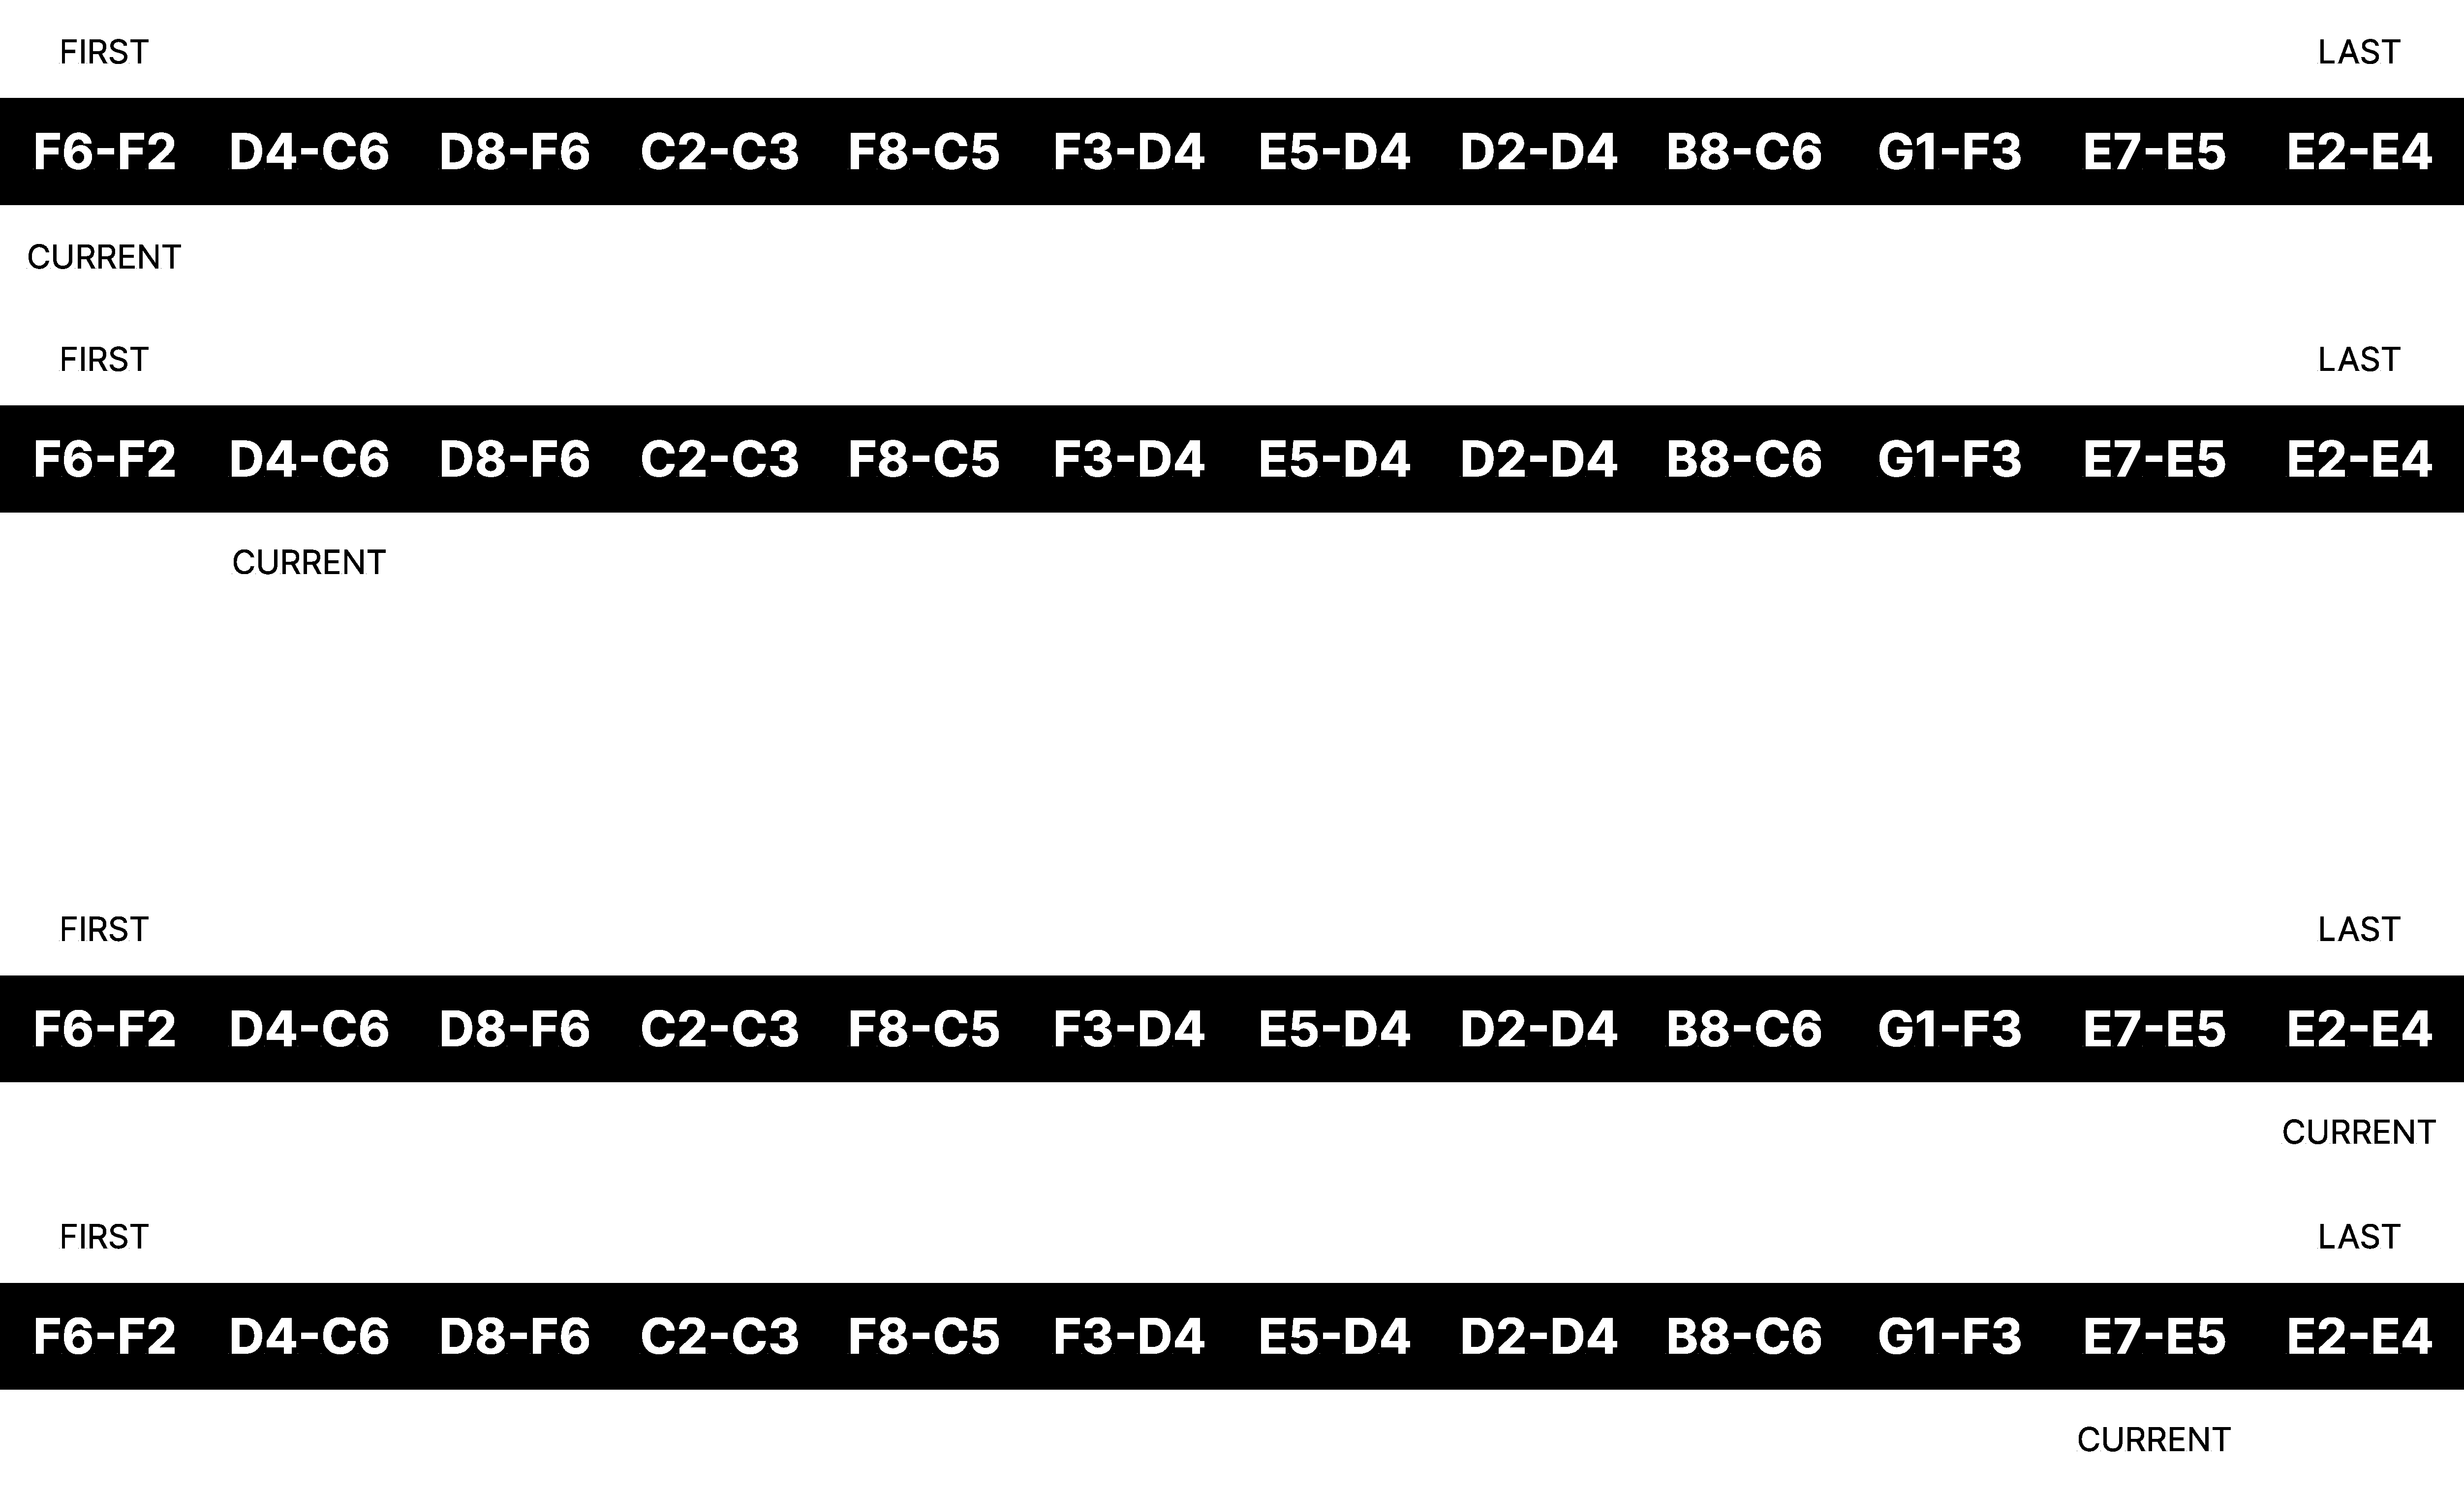
\includegraphics[width=1.0\textwidth]{figures/deque/chess-deque}
    \caption{Visual example of a deque with chess moves and a current index allowing element traversal from first-to-last (top two) and last-to-first (bottom two).}
    \label{fig:chess-deque}
\end{figure}

\section{Implementations of a deque}

The deque also has \sout{three} two implementations. Those implementations are similar to the queue's, but in the case of the array we access elements from two ends. Meanwhile the list implementation relies on doubly linked lists for both two-end access and traversal:

\begin{itemize}
    \item Doubly-linked lists
    \item Static arrays (not dynamic)
\end{itemize}

\subsection{The simple array}

The simplest implementation can include an array of objects and an index pointing to the current objects. To move through them, all that's needed is to increment/decrement the index. But what if the index is zero and decrementing causes the index to become negative, or even worse - underflow? The answer is simple, check if index is zero and then circle back, like this \(current = length - 1\). The simple array-based deque also needs to store the object count - deque length. Overflowing is fixed by checking if the current index is less than deque's length and doing the reverse, by making \(current = 0\). Visual example shown in \autoref{fig:array-deque}.

\begin{figure}
    \centering
    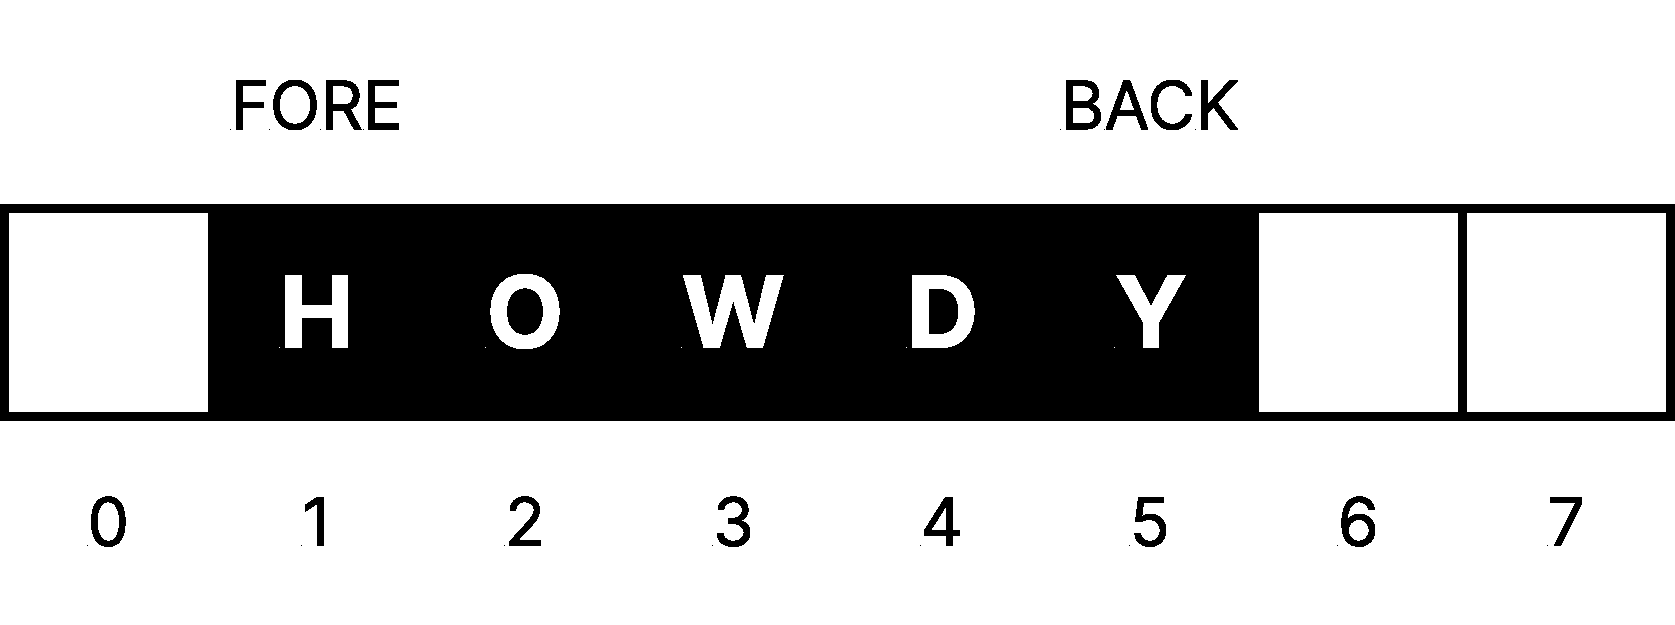
\includegraphics[width=0.7\textwidth]{figures/deque/array-deque}
    \caption{Visual example of an array-based deque with a current front (fore) index allowing element traversal from first-to-last (fore-to-back) and last-to-first (back-to-fore).}
    \label{fig:array-deque}
\end{figure}

\subsection{The complex doubly-linked list}

The most complex implementation can include linked list with one previous and one next pointer. To move through nodes simply get either the head (front) or tail (back) node and iterate through the entire list. To save memory we can make the list circular and only store the head node, since the tail will be accessible through head's previous node pointer, see \autoref{fig:list-deque}.

\begin{figure}
    \centering
    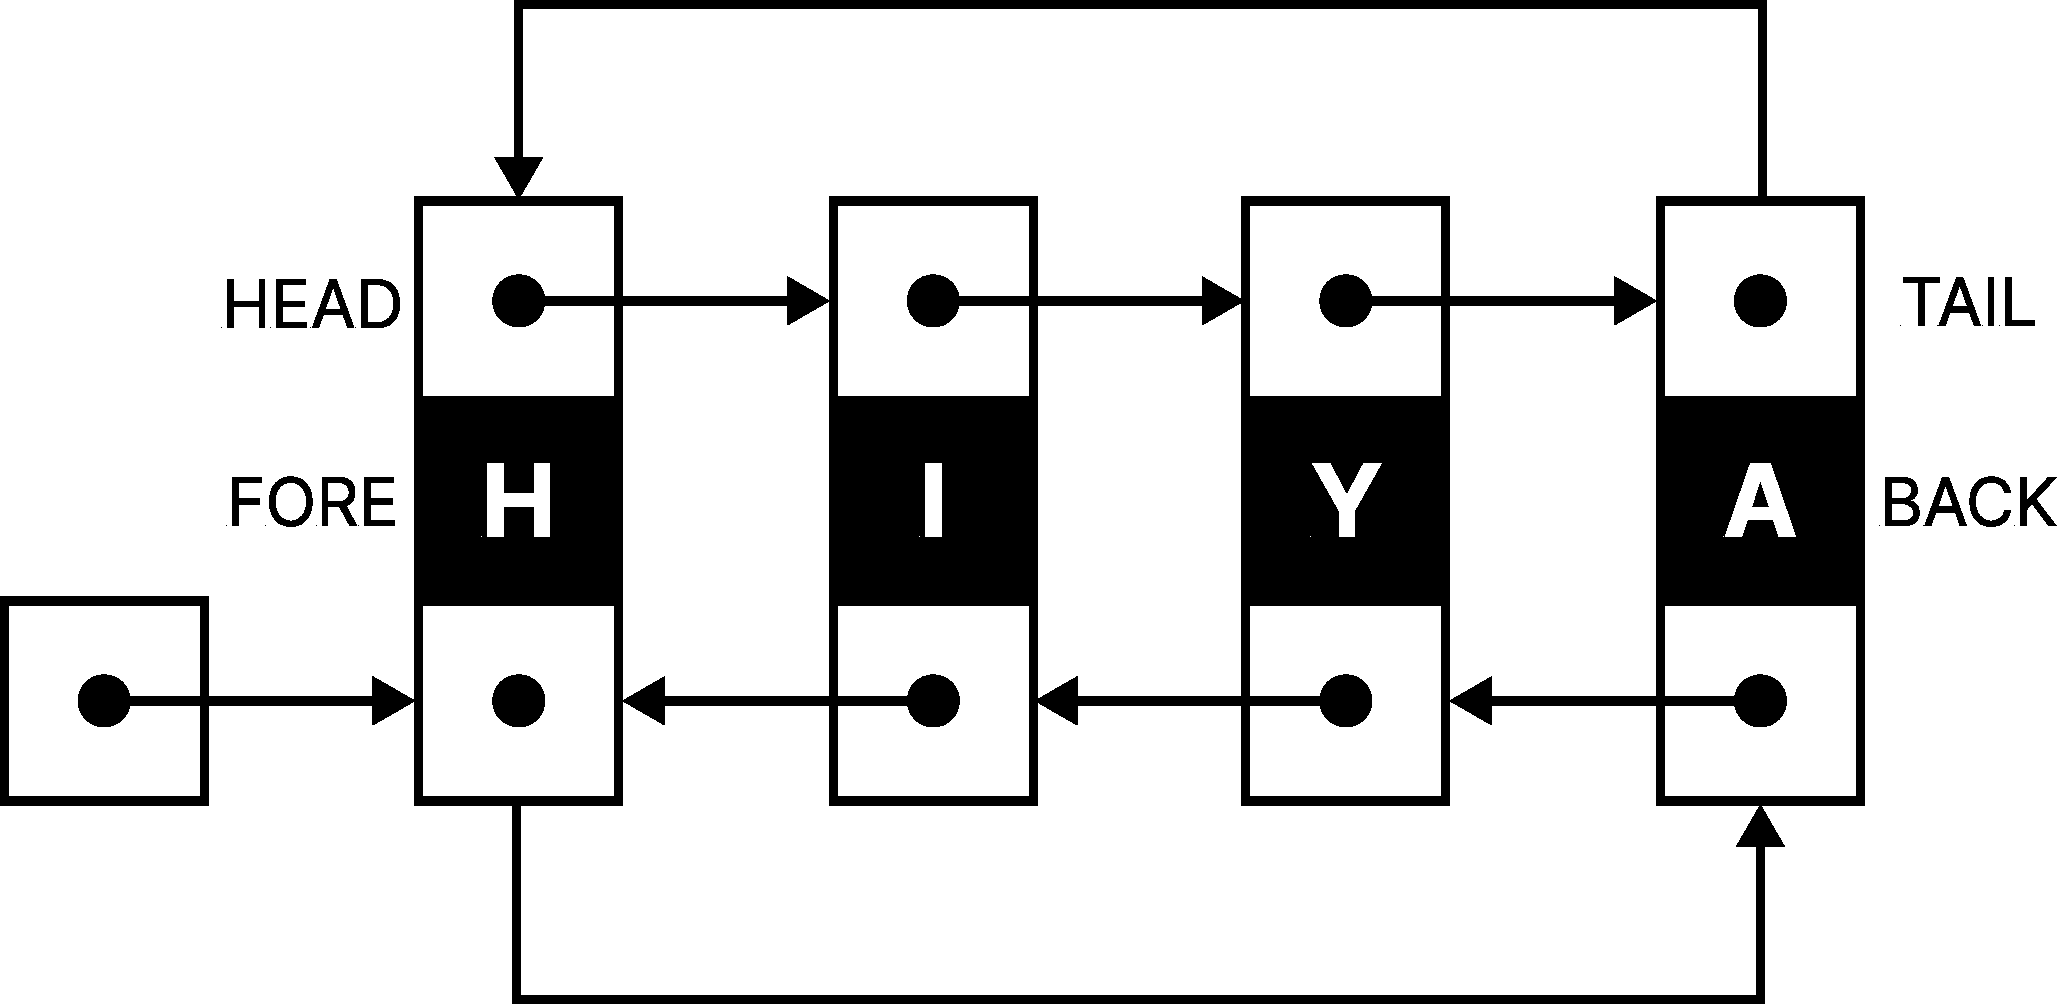
\includegraphics[width=0.7\textwidth]{figures/deque/list-deque}
    \caption{Visual example of a list-based deque with a current front (fore) head node allowing element traversal from first-to-last (fore-to-back) and last-to-first (back-to-fore).}
    \label{fig:list-deque}
\end{figure}

Another memory optimization for doubly-linked lists are XOR linked lists, which store the \texttt{next} and \texttt{previous} pointers as a single XOR pointer of the two, or more accurately, \(combined(A) = next(A) \oplus previous(A)\). To retrieve the next (or previous) node pointer, simply save the head (and tail) pointers as they are and XOR the head's (or tail's) combined pointer, like this \(next(A) = combined(A) \oplus previous(A)\). Again, to save memory we add more operations, but a drawback is that the list is harder to debug. C doesn't allow bitwise operations on pointers, but this can be avoided by casting the pointers to special integer types -- \texttt{intptr\_t} and \texttt{uintptr\_t}.

\begin{infobox}[title=Linux manual page - stdint.h(0p)]
The following type designates a signed integer type with the property that any valid pointer to void can be converted to this type, then converted back to a pointer to void, and the result will compare equal to the original pointer: \texttt{intptr\_t}
\newline
\newline
The following type designates an unsigned integer type with the property that any valid pointer to void can be converted to this type, then converted back to a pointer to void, and the result will compare equal to the original pointer: \texttt{uintptr\_t}
\end{infobox}

\subsection{Doubly-linked list of arrays}

Combining the properties of both lists and arrays I managed create a deque with good locality and growth, look at \autoref{fig:array-list-deque}. Each linked list node is made of a \texttt{previous} \texttt{next} and \text{elements\_array} member. Since it is this good is also gets described in more detail in the next section. Similar to the queue, this deque also relies on finding the perfect middle-ground between allocation speed (finding smaller memory chunks is faster) and locality (the bigger the memory array, the better the locality).

\begin{figure}
    \centering
    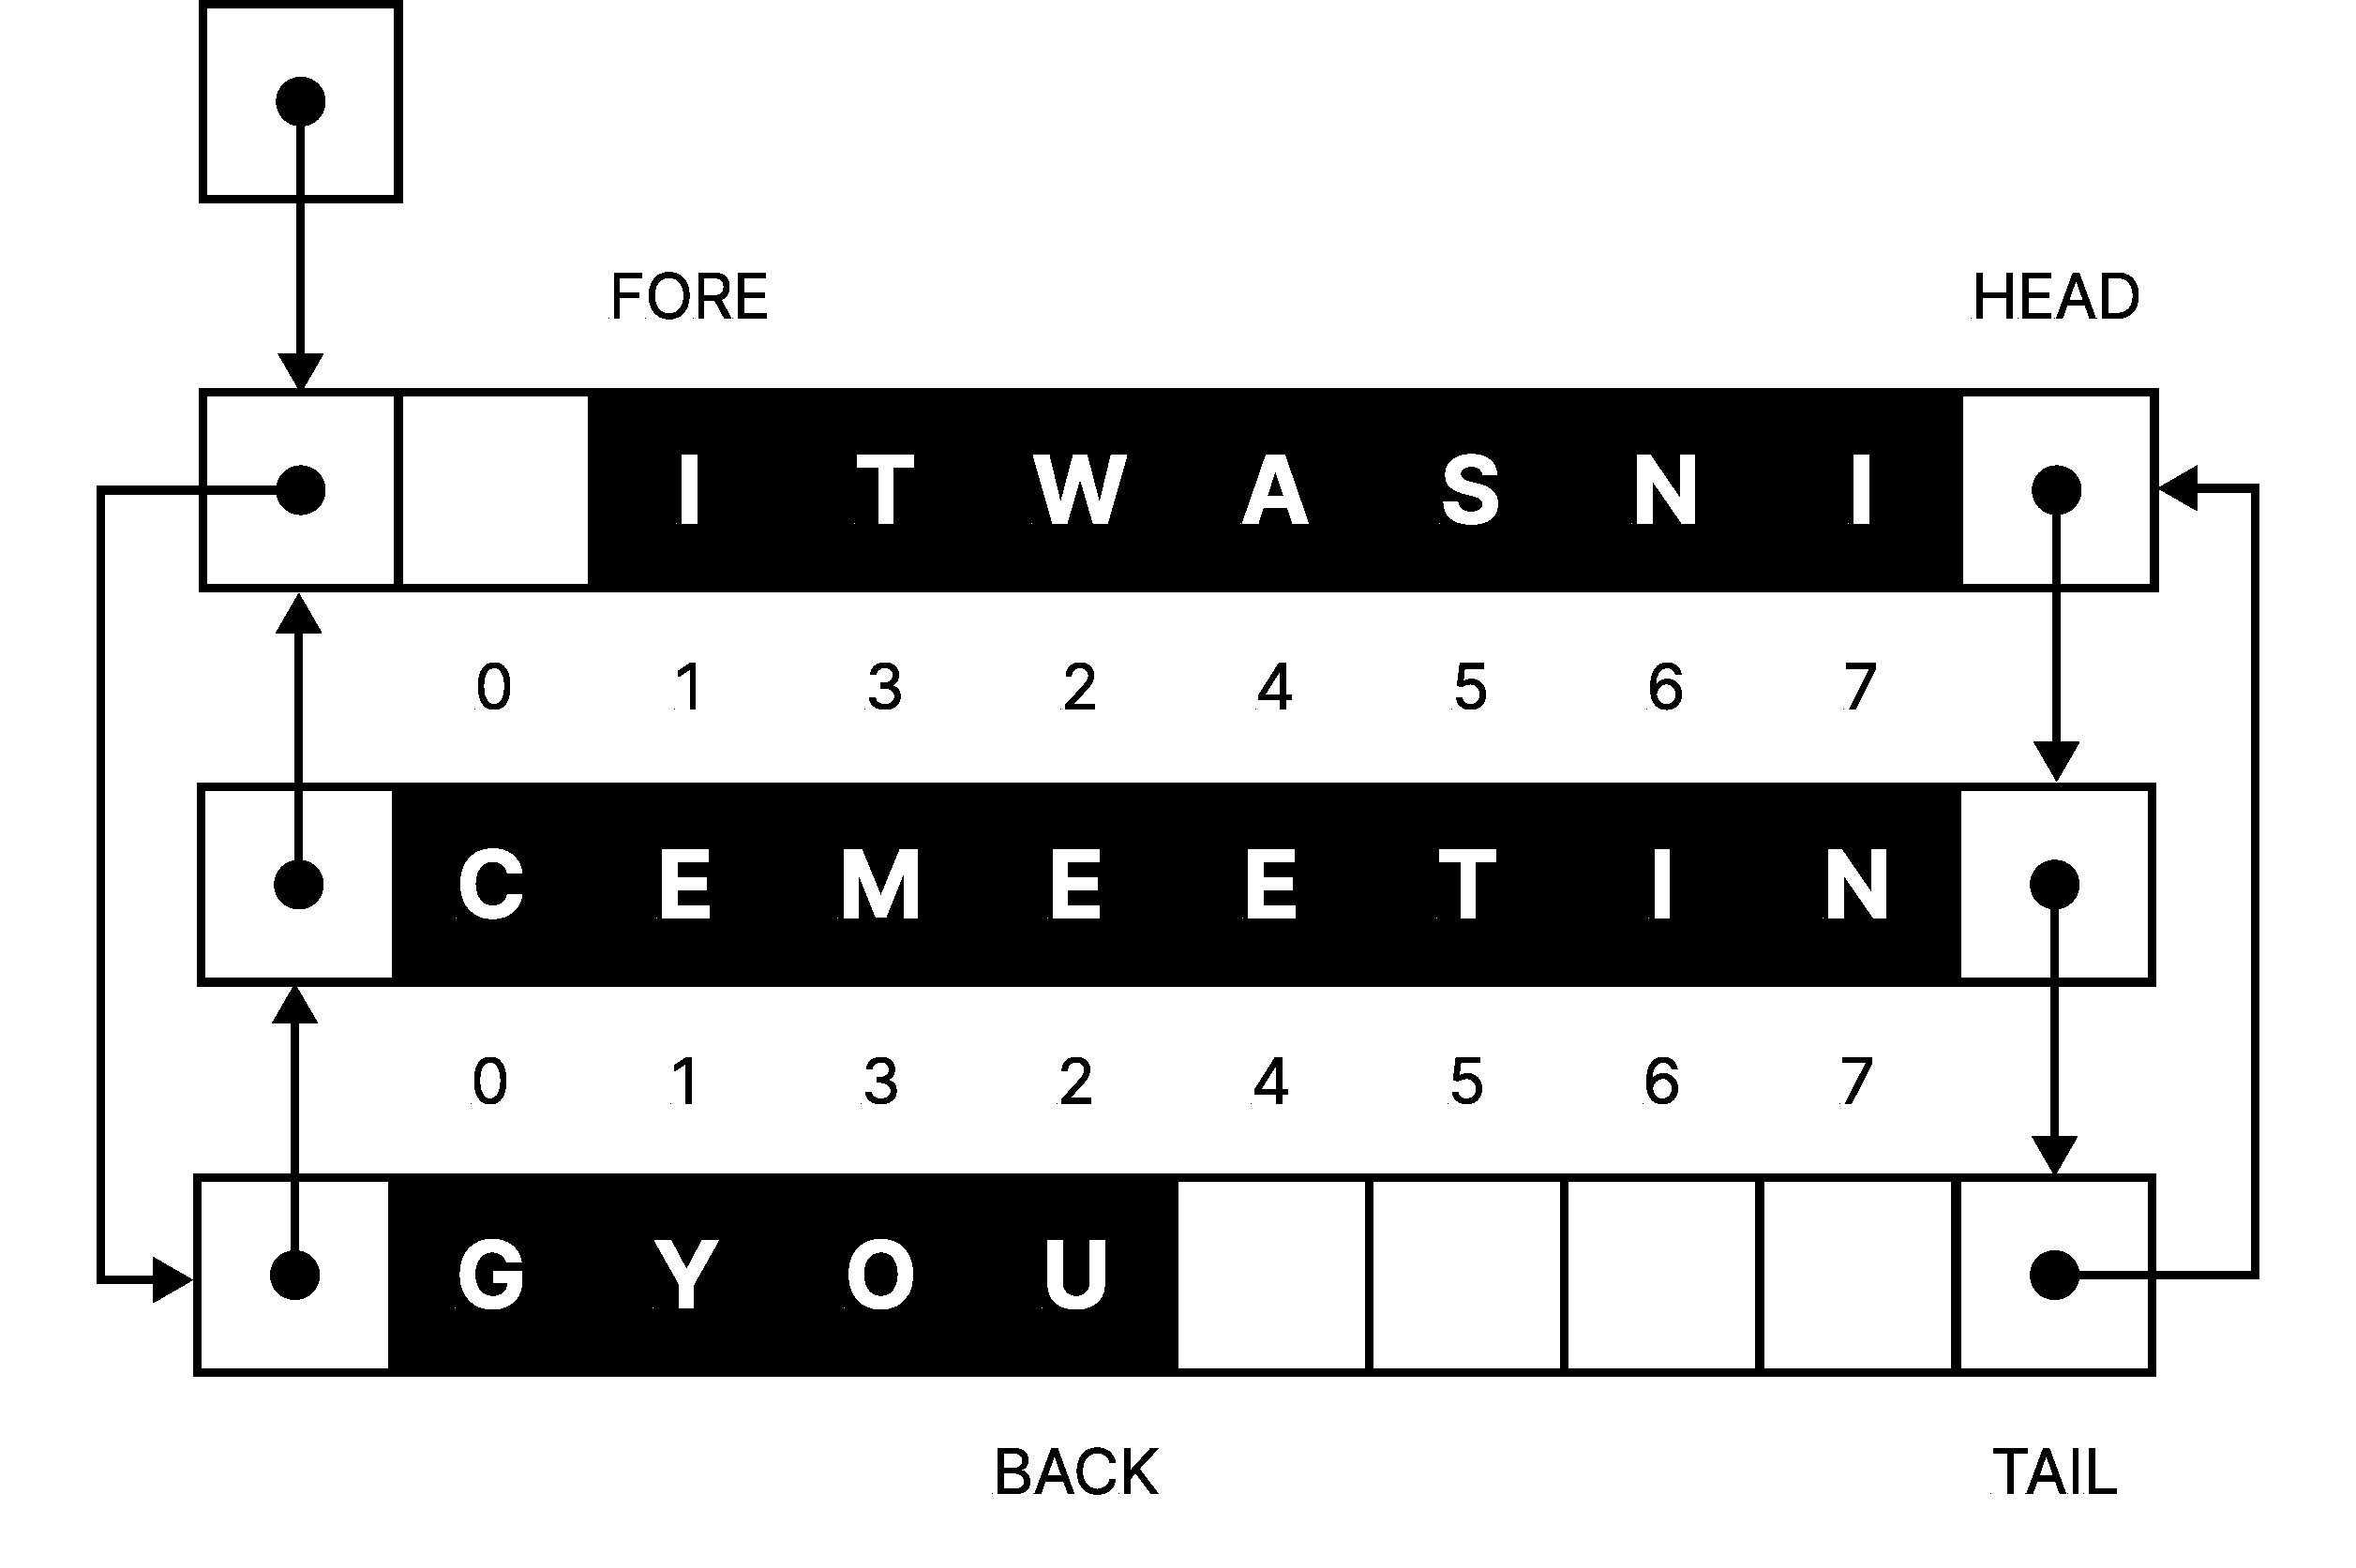
\includegraphics[width=0.7\textwidth]{figures/deque/array-list-deque}
    \caption{Visual example of an array-list based deque with a current front (fore) index allowing element traversal from first-to-last (fore-to-back) and last-to-first (back-to-fore).}
    \label{fig:array-list-deque}
\end{figure}

\subsection{The infinite deque structure}

The structure consists of a child node structure representing a doubly-linked list node with a flexible array member for storing elements.

The parent structure solely relies on the child head for element storage and traversal. The parent also stores the \texttt{current} front index to simplify front element access in \texttt{peek\_front\_ideque}. Next up is the \texttt{size} member storing individual element size, followed by \texttt{length}. \texttt{length} contains the number of elements in the deque. Lastly, the parent structure stores a pointer to a memory allocator structure for memory management.

\begin{lstlisting}[language=C, style=CodeEditor, label=lst:deque, title=include/sequence/ideque.h]
/// @brief Doubly linked list node for deque structure.
struct infinite_deque_node {
    struct infinite_deque_node * next; // next sibling node
    struct infinite_deque_node * prev; // previous sibling node
    char elements[];                   // elements array with IDEQUE_CHUNK size
};

/// @brief Inifnite deque data structure.
typedef struct infinite_deque {
    struct infinite_deque_node * head;
    size_t current, size, length; // current index, element size and structure length
    memory_s const * allocator;
} ideque_s;
\end{lstlisting}

\subsection{Create deque}

Creating a deque means only setting the \texttt{size} member to the size of the element type, and setting the \texttt{allocator} to the \texttt{standard} allocator pointer.

\begin{lstlisting}[language=C, style=CodeEditor, label=lst:create-deque, title=include/sequence/ideque.h]
/// @brief Creates an empty structure.
/// @param size Size of a single element
/// @return Deque structure.
ideque_s create_ideque(size_t const size);
\end{lstlisting}

\begin{lstlisting}[language=C, style=CodeEditor, label=lst:create-deque-01, title=include/sequence/ideque.c]
{
    \\ ...
    return (ideque_s) { .size = size, .allocator = allocator, };
}
\end{lstlisting}

\subsection{Make deque}

Making the structure is the same as creating it, but with the added option of using a custom memory allocator.

\begin{lstlisting}[language=C, style=CodeEditor, label=lst:make-deque, title=include/sequence/ideque.h]
/// @brief Creates a custom empty structure.
/// @param size Size of a single element.
/// @param allocator Custom allocator structure.
/// @return Deque structure.
ideque_s make_ideque(size_t const size, memory_s const * const allocator);
\end{lstlisting}

The memory allocator simply gets set to the \texttt{allocator} member of the structure, while the \texttt{size} member is set the same way as in \texttt{create\_ideque}.

\begin{lstlisting}[language=C, style=CodeEditor, label=lst:make-deque-01, title=include/sequence/ideque.c]
{
    \\ ...
    return (ideque_s) { .size = size, .allocator = allocator, };
}
\end{lstlisting}

\subsection{Destroy deque}

Destroying the deque means freeing each element using the \texttt{destroy} function pointer and its \texttt{ad} arguments. The destroy function pointer can either do nothing, set bytes in the element to zero or free the element if it is contains allocated memory.

\begin{lstlisting}[language=C, style=CodeEditor, label=lst:destroy-deque, title=include/sequence/ideque.h]
/// @brief Destroys a structure and its elements, but makes it unusable.
/// @param deque Structure to destroy.
/// @param destroy Function pointer to destroy a single element.
/// @param ad Arguments for destroy function pointer.
void destroy_ideque(ideque_s * const deque, set_fn const destroy, void * const ad);
\end{lstlisting}

First a current node pointer is initialized to the head node, then a for loop sets a \texttt{start} index for the current index position for the special case that a node has elements not at the start of the array. All the other nodes have therefore elements starting at index zero, hence the \texttt{start} variable is set to zero after the first iteration.

\begin{lstlisting}[language=C, style=CodeEditor, label=lst:destroy-deque-01, title=include/sequence/ideque.c]
{
    \\ ...
    struct infinite_deque_node * current = deque->head; // save head index as current node
    // for every node in deque list until size is not zero
    for (size_t start = deque->current, remaining = deque->length; remaining; start = 0) {
\end{lstlisting}

Following that, the index variable \texttt{i} is set to the \texttt{start} index, and a nested for loop iterates over the elements in the current node, destroying each element using the \texttt{destroy} function pointer. The loop continues until either all remaining elements have been destroyed or the end of the current node's elements array is reached. After destroying the elements, the \texttt{remaining} variable is updated to reflect the number of elements left to destroy.

\begin{lstlisting}[language=C, style=CodeEditor, label=lst:destroy-deque-02, title=include/sequence/ideque.c]
        size_t i = start; // set i outside of nested for loop to save its value
        for (; i < (remaining + start) && i < IDEQUE_CHUNK; ++i) { // destroy each element in node
            destroy(current->elements + (i * deque->size), ad);
        }
        remaining -= (i - start); // subtract absolute value of i and start from deque's size
\end{lstlisting}

Lastly, the current node is saved as a temporary variable \texttt{temp} for later freeing. Next the \texttt{current} node pointer is updated to point to the next node in the list. Finally, \texttt{temp} is freed using the defined memory allocator's \texttt{free} function.

\begin{lstlisting}[language=C, style=CodeEditor, label=lst:destroy-deque-03, title=include/sequence/ideque.c]
        struct infinite_deque_node * temp = current; // save current node as temporary to free later
        current = current->next; // go to next node

        deque->allocator->free(temp, deque->allocator->arg); // free temporary current node
    }
\end{lstlisting}

All that is left is to zero-out the deque structure, which is done by using \texttt{memset}.

\begin{lstlisting}[language=C, style=CodeEditor, label=lst:destroy-deque-04, title=include/sequence/ideque.c]

    // set everything to zero
    memset(deque, 0, sizeof(ideque_s));
}
\end{lstlisting}
